\chapter[Resultados obtenidos implementando un regulador experto.]{Resultados obtenidos implementando un regulador experto para controlar el diámetro}
\label{ane:resultados_regu}
\section{Ensayo 1}

\subsection{Condiciones del ensayo}

\begin{itemize}
	\item{Duración de experimento: 38 min}
	\item{Filamento extruido: 537 cm}
	\item{Granza de PLA mezcla: 70\% granza, 30\% pellets.}
	\item{Mezcla secada en horno 4 horas antes del ensayo.}
	\item{$T: 150^oC$}
	\item{$V_{min} tractora: 1.5 mm/s$}
	\item{$V_{max} tractora: 3.4 mm/s$}
	\item{Los incrementos de velocidades en las reglas del sistema experto son las mismas.}
\end{itemize}

\subsection{Resultados}
Cómo vemos en la Tabla \ref{tab:resl_ens1} la media del filamento conseguido es de $1.72 mm$, sin embargo, los valores límites de $1.65 mm$ y $1.85 mm$ han sido superados, por lo que el filamento que se ha extruido, no valdría en su totalidad para imprimir. Si representamos los datos obtenidos en una gráfica, podemos observar como hay una influencia del regulador. Las variaciones que hay en el diámetro, son no son tan pronunciadas como en el caso del funcionamiento en lazo abierto. \\

\begin{table}[H]
	\centering
	\begin{tabular}{cc}
		                    & Diámetro X \\ \hline
		Muestras            & 1526       \\
		Media (mm)          & 1.72       \\
		Desviación estandar & 0.29       \\
		Mínimo (mm)         & 1.20       \\
		Máximo (mm)         & 2.56      
	\end{tabular}
	\caption{Datos obtenidos en el ensayo 1}
	\label{tab:resl_ens1}
\end{table}


Con el gráfico de cajas, podemos ver que la distribución de los datos no es del todo homogena, teniendo una gran cantidad de los datos por encima de la media, sobre $1.96 mm$.

\begin{figure}[H]
    \centering
    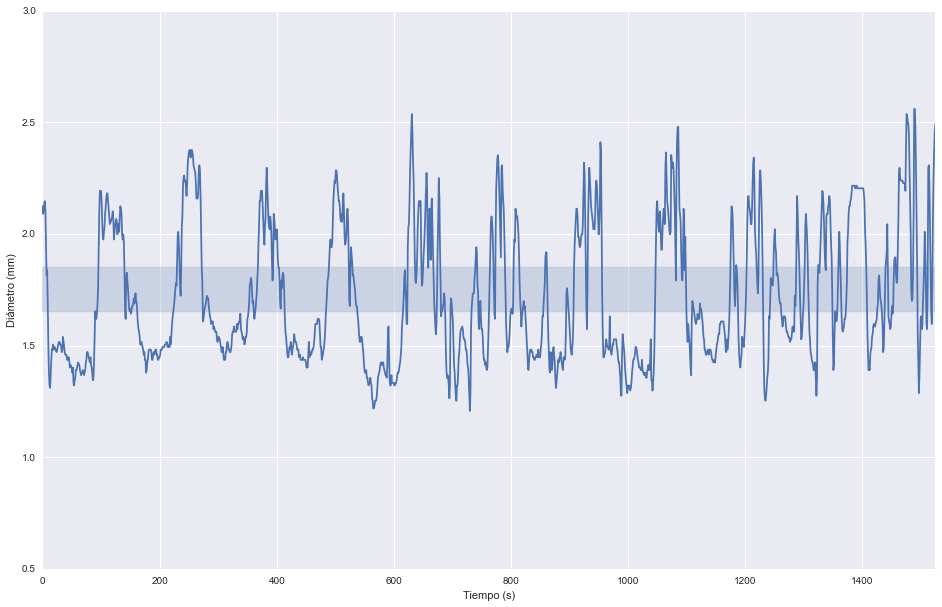
\includegraphics[width=0.99\textwidth]{images/producciones/11082015/output_9_1.png}
    \caption{Datos graficados del ensayo 1 con regulador experto}
    \label{fig:reg_graf1}
\end{figure}

\begin{figure}[H]
    \centering
    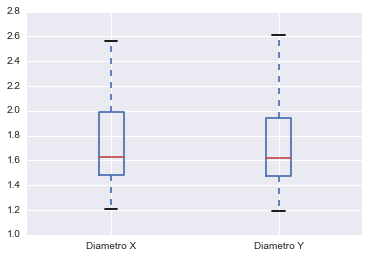
\includegraphics[width=0.6\textwidth]{images/producciones/11082015/output_10_1.png}
    \caption{Diagrama de cajas del ensayo 1 con regulador experto}
    \label{fig:reg_cajas1}
\end{figure}

Como segunda aproximación que vamos a realizar será la de hacer mayores incrementos al subir la velocidad en los tramos que el diámetro se encuentre entre $1.80 mm$ y $1.75 mm$ haremos incrementos de velocidad mayor.

\section{Ensayo 2}

\subsection{Condiciones del ensayo}

\begin{itemize}
	\item{Duración de experimento: 30 min}
	\item{Filamento extruido: 435cm}
	\item{Granza de PLA mezcla: 70\% granza, 30\% pellets.}
	\item{Mezcla secada en horno 4 horas antes del ensayo.}
	\item{$T: 150^oC$}
	\item{$V_{min} tractora: 1.5 mm/s$}
	\item{$V_{max} tractora: 3.4 mm/s$}
	\item{Los incrementos de velocidades en las reglas del sistema experto son distintas:}
\end{itemize}

En este ensayo, se va a cambiar el incremento de velocidad, cuando el filamento esté entre una diámetro de $1.75 mm$ y $1.80 mm$ y tenga una tendencia de crecimiento. Se hará que en este caso, la velocidad se incremente más.\\
\subsection{Resultados}
Los resultados obtenidos son los siguientes:

\begin{table}[H]
	\centering
	\begin{tabular}{cc}
		                    & Diámetro X \\ \hline
		Muestas             & 1114      \\
		Media (mm)          & 1.74       \\
		Desviación estandar & 0.26       \\
		Mínimo (mm)         & 1.02       \\
		Máximo (mm)         & 2.45      
	\end{tabular}
	\caption{Datos obtenidos en el ensayo 2}
	\label{tab:resl_ens2}
\end{table}

Con los cambios realizados, los datos ahora son algo más estables, y hemos conseguido aumentar la media del filamento a $1.74 mm$ estando dentro del margen de producción, sin embargo, los límites superior e inferior no son los adecuados, alejándose demasiado de lo deseado. Sin embargo en este caso, una gran parte del filamento podría llegar a ser re-aprovechado para imprimir.

\begin{figure}[H]
    \centering
    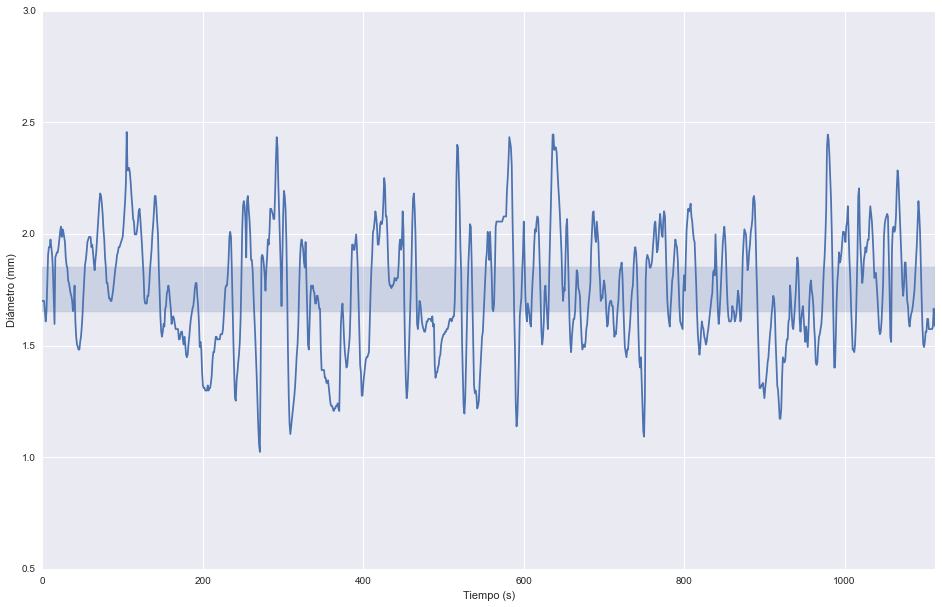
\includegraphics[width=0.99\textwidth]{images/producciones/12082015/output_9_e1.png}
    \caption{Datos graficados del ensayo 2 con regulador experto}
    \label{fig:reg_graf2}
\end{figure}

\begin{figure}[H]
    \centering
    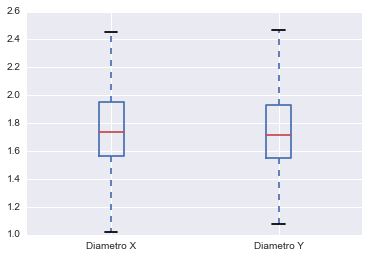
\includegraphics[width=0.6\textwidth]{images/producciones/12082015/output_10_e1.png}
    \caption{Diagrama de cajas del ensayo 2 con regulador experto}
    \label{fig:reg_cajas2}
\end{figure}

Como tercera aproximación, vamos a modificar los incrementos de velocidades en los tramos en los que el filamento se encuentre entre  $1.70 mm$ y $1.80 mm$

\section{Ensayo 3}

\subsection{Condiciones del ensayo}

\begin{itemize}
	\item{Duración de experimento: 30min}
	\item{Filamento extruido: 425cm}
	\item{Granza de PLA mezcla: 70\% granza, 30\% pellets.}
	\item{Mezcla secada en horno 4 horas antes del ensayo.}
	\item{$T: 150^oC$}
	\item{$V_{min} tractora: 1.5 mm/s$}
	\item{$V_{max} tractora: 3.4 mm/s$}
	\item{Los incrementos de velocidades en las reglas del sistema experto son distintas:}
\end{itemize}

En este ensayo, se va a cambiar el incremento de velocidad, cuando el filamento esté entre una diámetro de $1.75 mm$ y $1.80 mm$ y sea cual sea la tendencia. Se hará que en este caso, la velocidad se incremente más.\\
\subsection{Resultados}
Los resultados obtenidos son los siguientes:

\begin{table}[H]
	\centering
	\begin{tabular}{cc}
		                    & Diámetro X \\ \hline
		Medidas             & 1124      \\
		Media (mm)          & 1.66       \\
		Desviación estandar & 0.24       \\
		Mínimo (mm)         & 0.98       \\
		Máximo (mm)         & 2.60      
	\end{tabular}
	\caption{Datos obtenidos en el ensayo 3}
	\label{tab:resl_ens3}
\end{table}

Con esta tercera aproximación se ha conseguido estabilizar los datos y reducir la desviación estandar, sin embargo, la media del filamento y de la velocidad de tracción ha disminuido también. Por lo tanto, los cambios realizados no han sido satisfactorio

\begin{figure}[H]
    \centering
    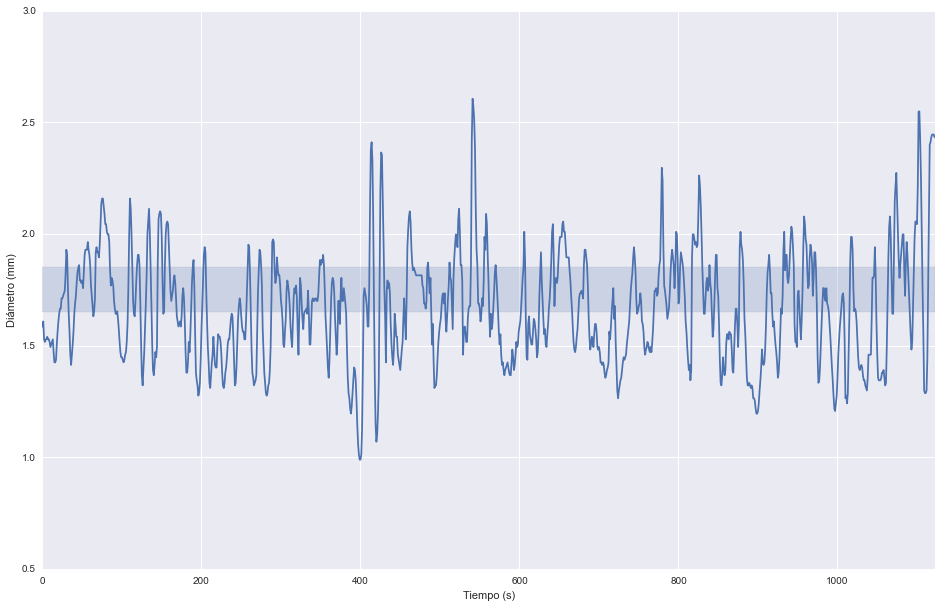
\includegraphics[width=0.99\textwidth]{images/producciones/12082015/output_9_e2.png}
    \caption{Datos graficados del ensayo 3 con regulador experto}
    \label{fig:reg_graf3}
\end{figure}

\begin{figure}[H]
    \centering
    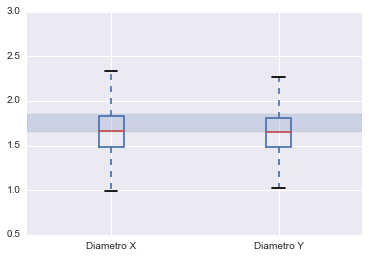
\includegraphics[width=0.6\textwidth]{images/producciones/12082015/output_10_e2.png}
    \caption{Diagrama de cajas del ensayo 3 con regulador experto}
    \label{fig:reg_cajas3}
\end{figure}

Como cuarta  aproximación, vamos a  modificar los incrementos en los que el diámetro se encuentra entre $1.70 mm$ y $1.80 mm$, en sentido de subida. En el sentido de bajada se mantendrá con incrementos de +1.\\

Se ha detectado también que el eje de giro de la tractora está algo suelto. Se va a apretar para el siguiente ensayo.\\

\section{Ensayo 4}
\label{lab:4} 
\subsection{Condiciones del ensayo}
Los datos con los que se realizaron el experimento fueron:

\begin{itemize}
	\item{Duración de experimento: 30min}
	\item{Filamento extruido: 447cm}
	\item{Granza de PLA mezcla: 70\% granza, 30\% pellets.}
	\item{Mezcla secada en horno 4 horas antes del ensayo.}
	\item{$T: 150^oC$}
	\item{$V_{min} tractora: 1.5 mm/s$}
	\item{$V_{max} tractora: 3.4 mm/s$}
	\item{Los incrementos de velocidades en las reglas del sistema experto son distintas.}
\end{itemize}

 Los tramos entre $1.70 mm$ y $1.80mm$ en los que haya una tendencia a aumentar, se incrementará la velocidad, sin embargo cuando se tenga una tendencia a disminuir, se volverá a tener una incremento de velocidad de +1.\\
\subsection{Resultados}
Los resultados obtenidos son los siguientes:

\begin{table}[H]
	\centering
	\begin{tabular}{cc}
		                    & Diámetro X \\ \hline
		Medidas             & 1125      \\
		Media (mm)          & 1.71       \\
		Desviación estandar & 0.23       \\
		Mínimo (mm)         & 1.01       \\
		Máximo (mm)         & 2.30      
	\end{tabular}
	\caption{Datos obtenidos en el ensayo 4}
	\label{tab:resl_ens4}
\end{table}

Con esta tercera aproximación se ha conseguido estabilizar los datos y reducir la desviación estandar, sin embargo, la media del filamento y de la velocidad de tracción ha disminuido también. Por lo tanto, los cambios realizados no han sido satisfactorio

\begin{figure}[H]
    \centering
    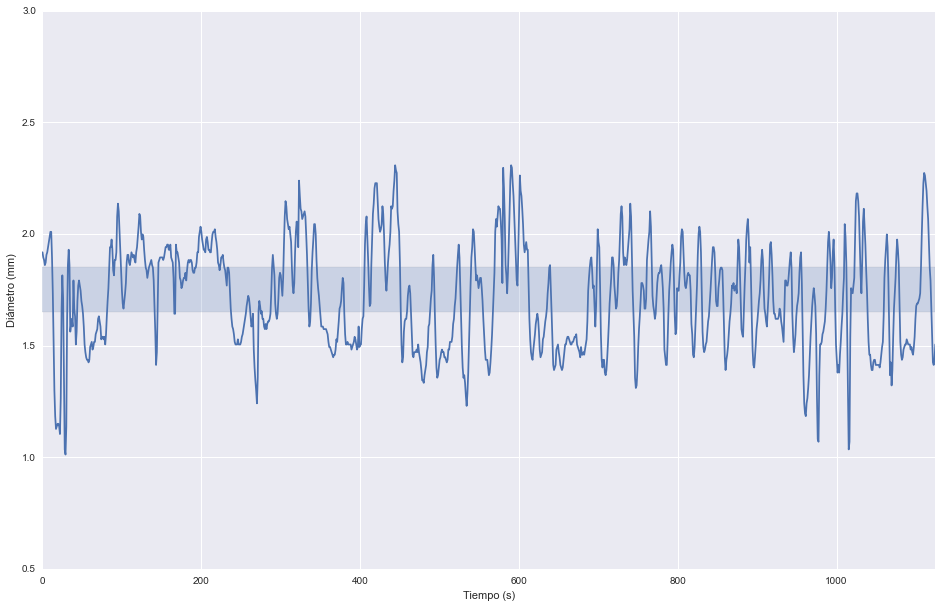
\includegraphics[width=0.99\textwidth]{images/producciones/13082015/output_9_e1.png}
    \caption{Datos graficados del ensayo 4 con regulador experto}
    \label{fig:reg_graf4}
\end{figure}

\begin{figure}[H]
    \centering
    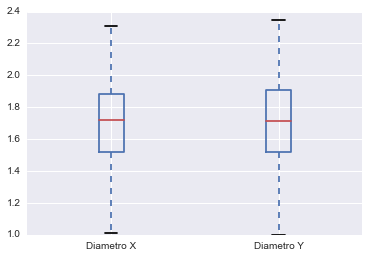
\includegraphics[width=0.6\textwidth]{images/producciones/13082015/output_10_e1.png}
    \caption{Diagrama de cajas del ensayo 4 con regulador experto}
    \label{fig:reg_cajas4}
\end{figure}

Como quinta  aproximación, vamos a  modificar los rangos de velocidades de la tractora. Vamos a pasar a unas velocidades de $1.5RPM$ a $5.3RPM$ \\

\section{Ensayo 5}
\subsection{Condiciones del ensayo}
Los datos con los que se realizaron el experimento fueron:

\begin{itemize}
	\item{Duración de experimento: 20min}
	\item{Filamento extruido: 314cm}
	\item{Granza de PLA mezcla: 70\% granza, 30\% pellets.}
	\item{Mezcla secada en horno 4 horas antes del ensayo.}
	\item{$T: 150^oC$}
	\item{$V_{min} tractora: 1.5 mm/s$}
	\item{$V_{max} tractora: 5.3 mm/s$}
	\item{Los incrementos de velocidades en las reglas del sistema experto son distintas.}
\end{itemize}

Este experimento sólo dura 20min, debido a que durante la realización del mismo, se percibe que no aporta ninguna mejora, añadiendo más inestabilidad a la medidas.\\

\subsection{Resultados}

\begin{table}[H]
	\centering
	\begin{tabular}{cc}
		                    & Diámetro X \\ \hline
		Medidas             & 750      \\
		Media (mm)          & 1.43       \\
		Desviación estandar & 0.36       \\
		Mínimo (mm)         & 0.00       \\
		Máximo (mm)         & 2.31      
	\end{tabular}
	\caption{Datos obtenidos en el ensayo 5}
	\label{tab:resl_ens5}
\end{table}

\begin{figure}[H]
    \centering
    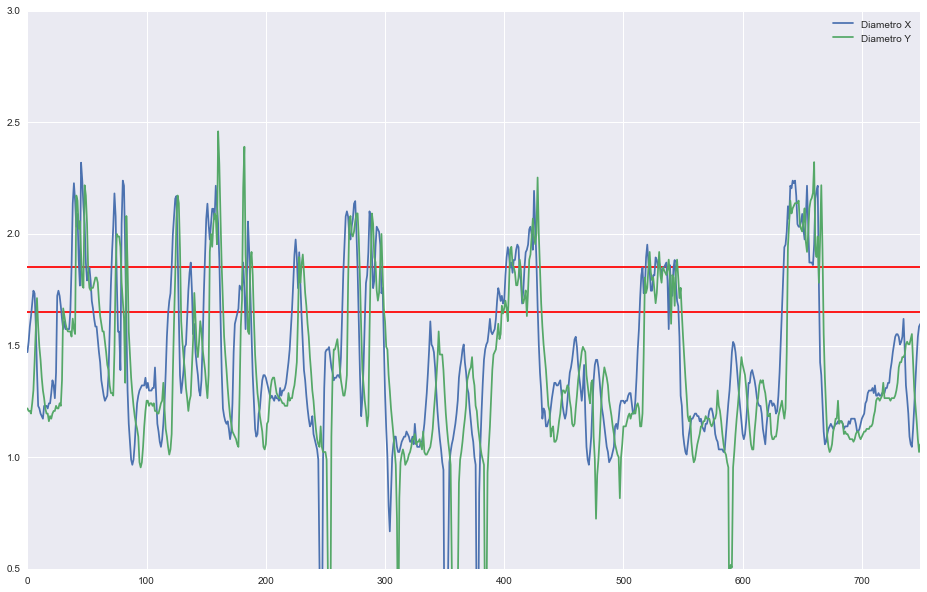
\includegraphics[width=0.99\textwidth]{images/producciones/13082015/output_9_e2.png}
    \caption{Datos graficados del ensayo 5 con regulador experto}
    \label{fig:reg_graf5}
\end{figure}

\begin{figure}[H]
    \centering
    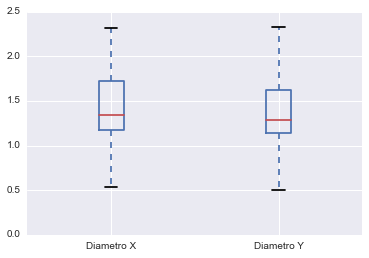
\includegraphics[width=0.6\textwidth]{images/producciones/13082015/output_10_e2.png}
    \caption{Diagrama de cajas del ensayo 5 con regulador experto}
    \label{fig:reg_cajas5}
\end{figure}

Aumentando la velocidad se ha conseguido que disminuya el valor máximo, sin embargo ha disminuido el valor mínimo. Para la siguiente iteracción, se va a volver a las velocidades de $1.5RPM$ - $3.4RPM$ y se van a añadir más reglas con unos incrementos de velocidades menores, para evitar saturar la velocidad de traccción tanto a nivel alto como nivel bajo.

\section{Ensayo 6}
\subsection{Condiciones del ensayo}


\begin{itemize}
	\item{Duración de experimento: 30min}
	\item{Filamento extruido: 453cm}
	\item{Granza de PLA mezcla: 70\% granza, 30\% pellets.}
	\item{Mezcla secada en horno 4 horas antes del ensayo.}
	\item{$T: 150^oC$}
	\item{$V_{min} tractora: 1.5 mm/s$}
	\item{$V_{max} tractora: 3.4 mm/s$}
	\item{Los incrementos de velocidades en las reglas del sistema experto son distintas.}
\end{itemize}

 Los tramos entre $1.70 mm$ y $1.80mm$ en los que haya una tendencia a aumentar, se incrementará la velocidad, sin embargo cuando se tenga una tendencia a disminuir, se tendrá una incremento de velocidad de +1.\\
\subsection{Resultados}
Los resultados obtenidos son los siguientes:

\begin{table}[H]
	\centering
	\begin{tabular}{cc}
		                    & Diámetro X \\ \hline
		Medidas             & 1087      \\
		Media (mm)          & 1.71       \\
		Desviación estandar & 0.26       \\
		Mínimo (mm)         & 1.05       \\
		Máximo (mm)         & 2.44      
	\end{tabular}
	\caption{Datos obtenidos en el ensayo 6}
	\label{tab:resl_ens6}
\end{table}

Con esta tercera aproximación se ha conseguido estabilizar los datos y reducir la desviación estandar, sin embargo, la media del filamento y de la velocidad de tracción ha disminuido también. Por lo tanto, los cambios realizados no han sido satisfactorio

\begin{figure}[H]
    \centering
    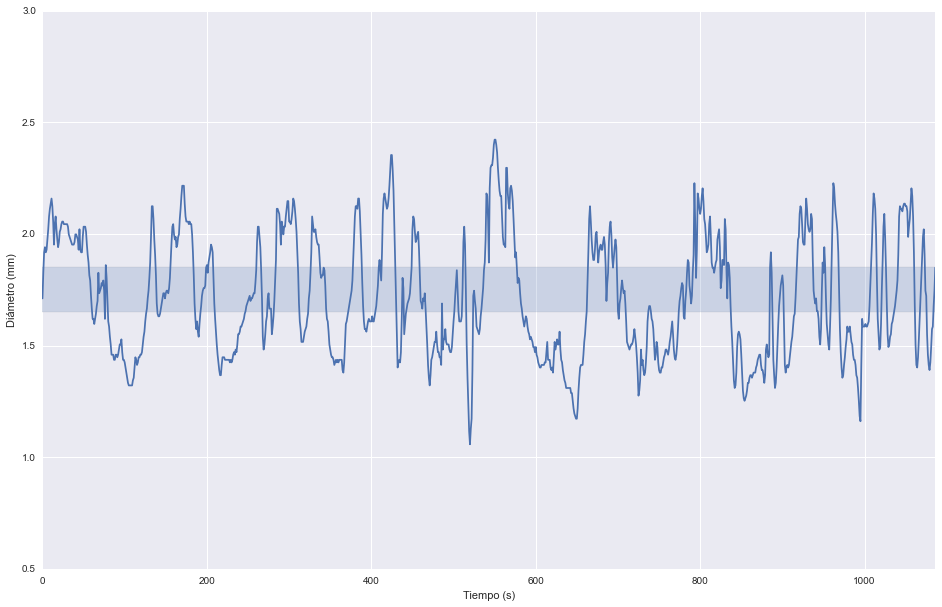
\includegraphics[width=0.99\textwidth]{images/producciones/13082015/output_9_e3.png}
    \caption{Datos graficados del ensayo 6 con regulador experto}
    \label{fig:reg_graf6}
\end{figure}

\begin{figure}[H]
    \centering
    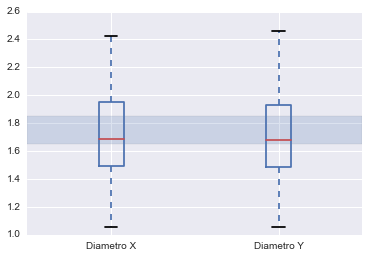
\includegraphics[width=0.6\textwidth]{images/producciones/13082015/output_10_e3.png}
    \caption{Diagrama de cajas del ensayo 6 con regulador experto}
    \label{fig:reg_cajas6}
\end{figure}

\section{Conclusiones}

Después de realizar los seis experimentos, la tabla \ref{tab:_results} muestra los resultados en cada uno de ellos.\\

\begin{table}[H]
	\centering
	\begin{tabular}{lccccccc}
		                    &Lazo Abierto     & Ensayo 1 & Ensayo 2 & Ensayo 3 & Ensayo 4 & Ensayo 5 & Ensayo 6 \\ \hline
		Medidas             &     203         & 1526     & 1114     & 1124     & 1125     & 750      & 1087     \\
		Media (mm)          &	1.59		 & 1.72     & 1.74     & 1.66     & 1.71     & 1.43     & 1.71     \\
		Desviación estandar &	0.25		 & 0.29     & 0.26     & 0.24     & 0.23     & 0.36     & 0.26     \\
		min(mm)             &	1.08		 & 1.20     & 1.02     & 0.98     & 1.01     & 0        & 1.05     \\
		max(mm)             &	2.19		 & 2.56     & 2.45     & 2.60     & 2.30     & 2.31     & 2.44    
	\end{tabular}
	\caption[Tabla comparativa de los resultados obtenidos.]{Tabla comparativa de los resultados obtenidos. Observamos la influencia del regulador contra el sistema en lazo abierto.}
	\label{tab:_results}
\end{table}

Como podemos comprobar, hemos conseguido tener un diámetro, cuyo valor medio está dentro de los márgenes de teolerancia, sin embargo, los valores máximos y mínimos no cumplen los requisitos. Esto es debido a que el filamento no sale de manera constante de la extrusora y por ello, el control del mismo, se hace más complicado si cabe. Sin embaego, hemos podido comprobar como el regulador que hemos implementado aplica una cierta mejora respecto al extrusor en lazo abierto.\\
